\documentclass[AdvProjMgmt_Sebastien_Deriaz]{subfiles}


\begin{document}
\section{Concept of operations}
\begin{figure}[H]
\centering
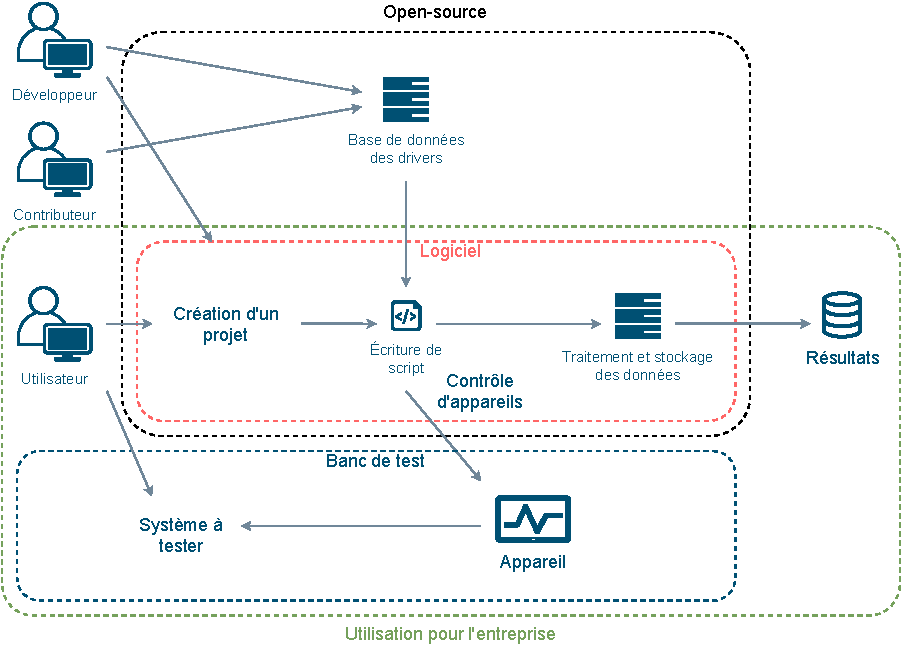
\includegraphics[scale=1]{schema_conops.pdf}
\end{figure}
Le ConOps\footnote{Concept of Operations} mets en évidences les acteurs principaux du projet :
\begin{enumerate}
\item Développeur
\item Contributeur
\item Utilisateur
\end{enumerate}
L'utilisateur va se servir du logiciel afin de réaliser des tests (sur un matériel et un système qui lui appartiennent et sur lesquels le développeur et le contributeur n'ont pas d'impact). Au travers de ses tests et mesures, l'utilisateur va créer des données dont le traitement et le stockage sont sous sa responsabilité.\\
Le développeur se charge de fournir un programme fonctionnel, qui répond au mieux aux besoins du client.\\
Le contributeur fournit un service bénévole permettant d'étendre les capacités du système (compatibilité avec plus d'appareils par exemple).\\
Le workflow typique de l'utilisateur consiste en :
\begin{enumerate}
\item Création d'un projet
\item Écriture de code (script) permettant d'effectuer les tests et mesures dont il a besoin
\item Traitement et stockage des données
\item Publication et utilisation des données au sein de l'entreprise.
\end{enumerate}







\end{document} 